\section{Evaluaci�n de recursos}

\subsection{planificaci�n}
La planificaci�n inicial del proyecto ha sido realizada mediante el software OpenProj para Mac Os X. A continuaci�n se muestran los resultados de la planificaci�n.
% \newpage{\pagestyle{empty}\cleardoublepage} 
   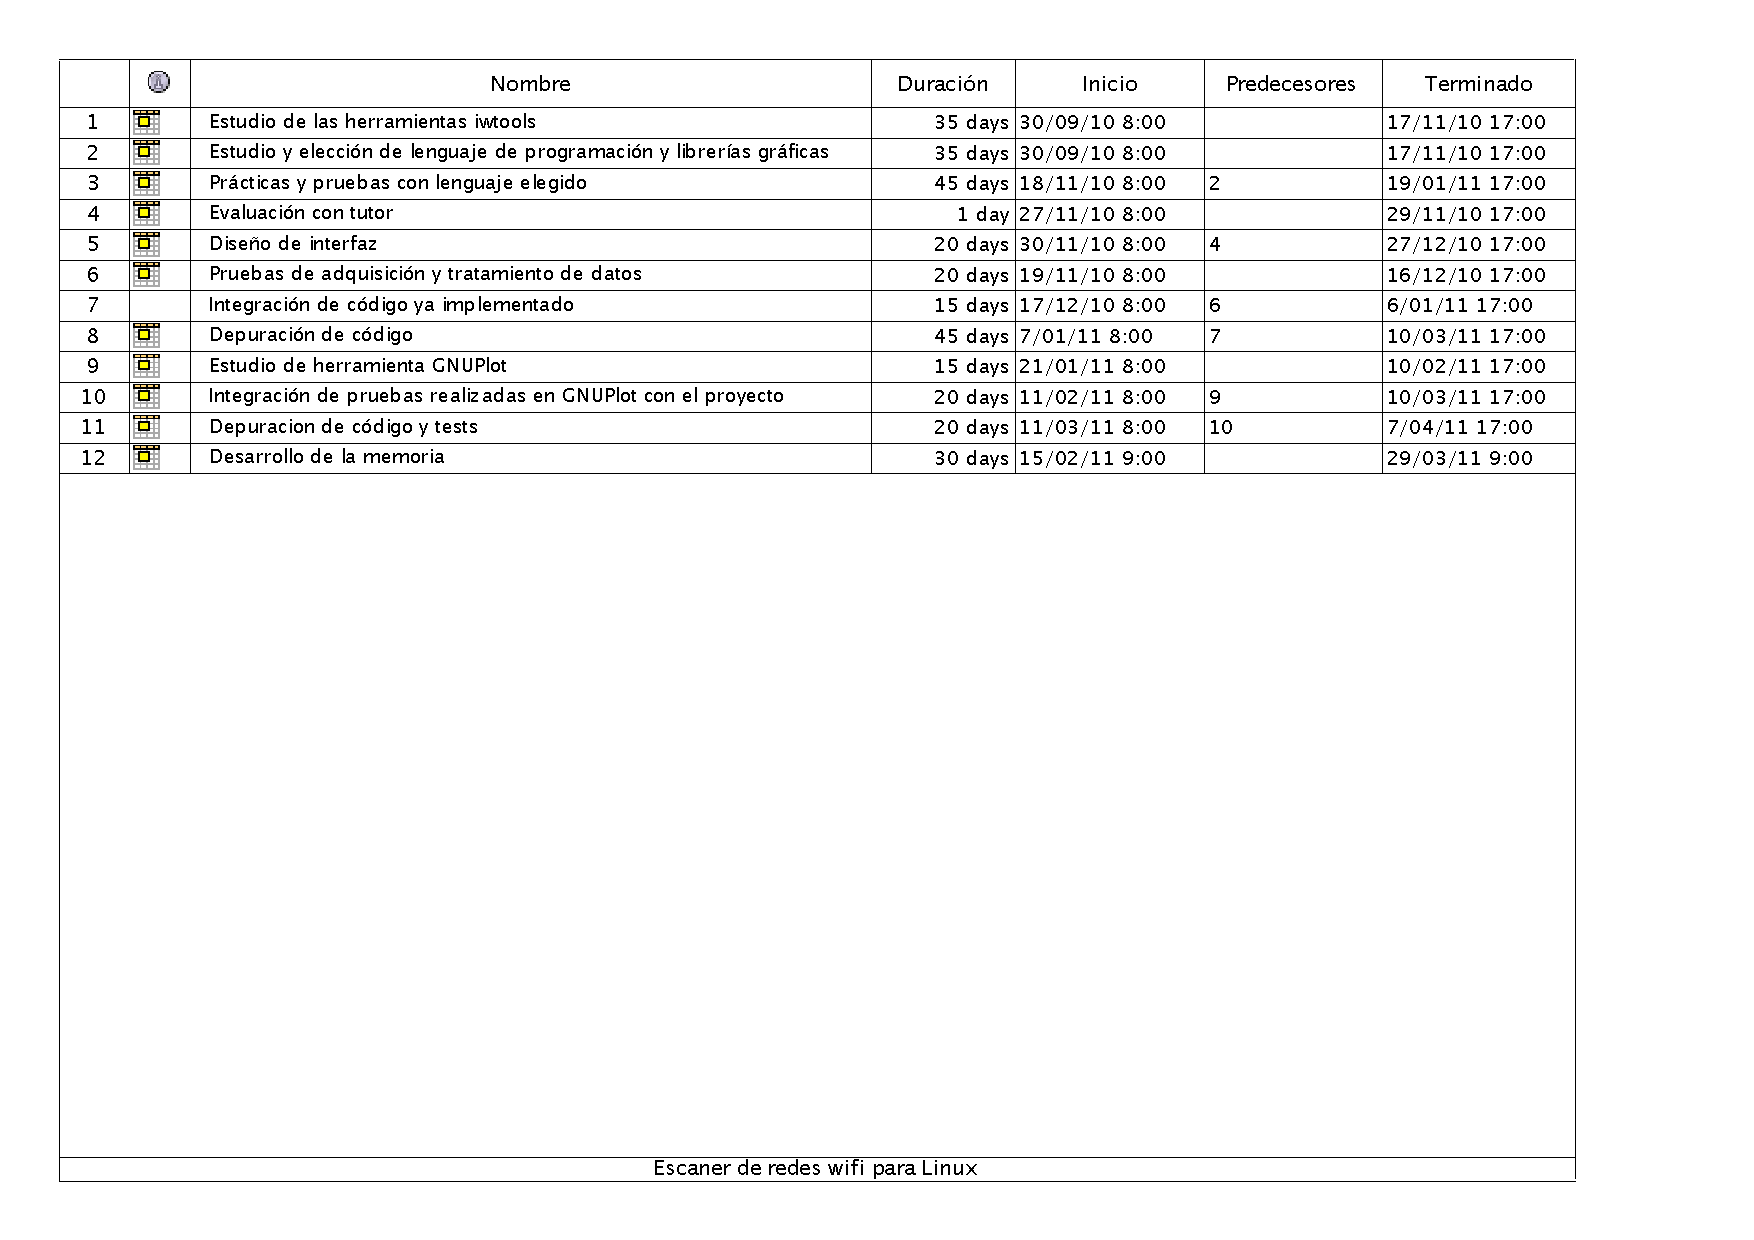
\includepdf[]{src/planificacion_por_hitos.pdf}
 \newpage{\pagestyle{empty}\cleardoublepage} 
    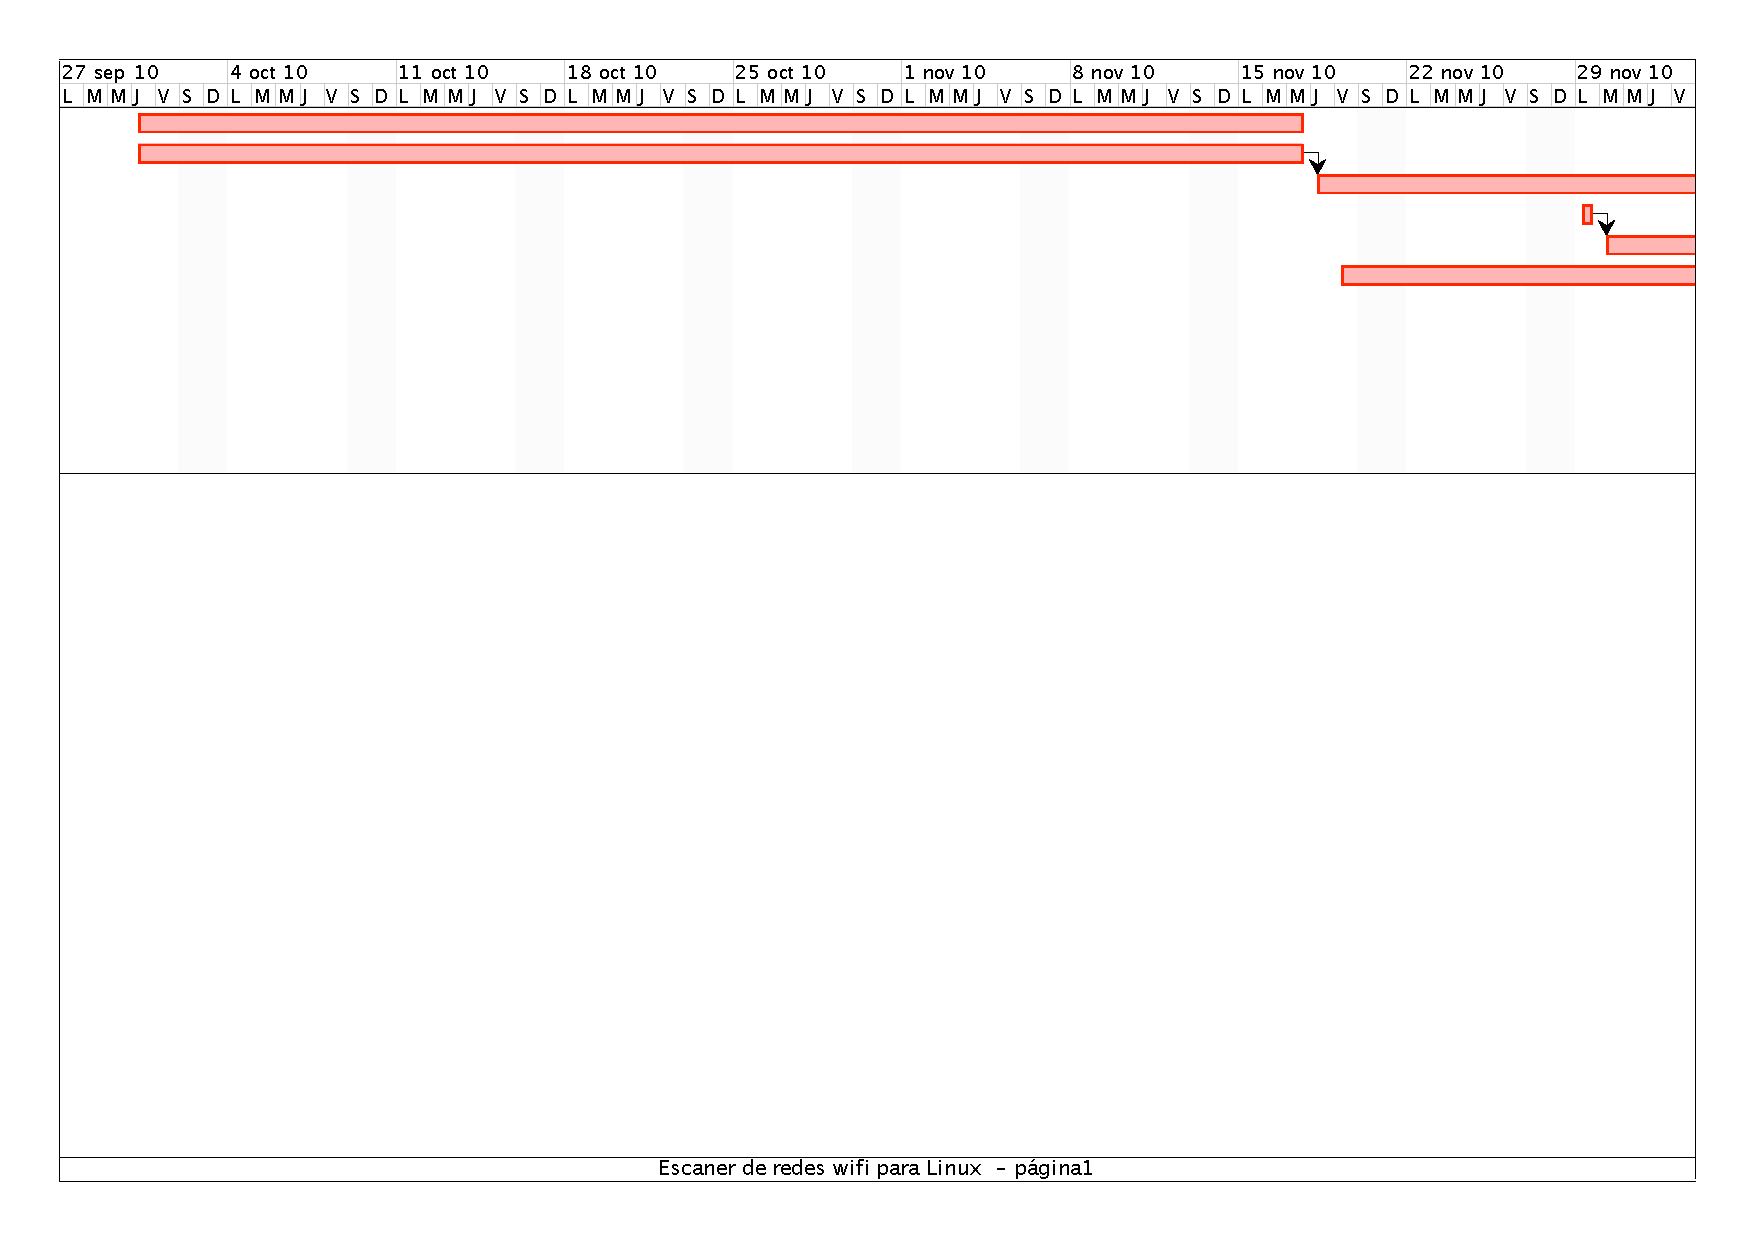
\includepdf[pages={1-3}, landscape]{src/planificacion_gantt.pdf}
 \newpage{\pagestyle{empty}\cleardoublepage} 

\section*{Presupuesto}

A partir de la duraci�n prevista de las tareas a realizar y el coste de los materiales utilizados, se puede obtener el coste de desarrollo del proyecto. Este coste ser� aproximado ya que es previo a la realizaci�n del mismo.\\

Un coste importante es el que deriva del sueldo de los trabajadores implicados en �l. En este caso, se trata de un �nico trabajador (el alumno). Para determinar el sueldo de este trabajador, se supone que se trata de un ingeniero t�cnico ya que es la titulaci�n en la cual se est� desarrollando el proyecto. Esto explica por qu� se ha planificado en 180 d�as (6 meses) y no en 90.\\

El sueldo mensual de un ingeniero t�cnico se supondr� de 1200 euros a jornada completa de 8 horas. Por lo tanto el trabajador ganar�a en torno a los 7.5 euros/hora. Este proyecto se ha realizado a media jornada,debido a la compaginaci�n con otros trabajos.\\

Con este c�lculo, se puede obtener el sueldo total del trabajador teniendo sabiendo que el proyecto tendr� una duraci�n de 720 horas. \\
720 x 7.5 = 5400\euro . Este ser� el sueldo del trabajador.

Tomando �ste proyecto desde cero, la inversi�n f�sica a realizar no es muy elevada. Se comenz� el desarrollo en un pc obsoleto, sin conexi�n v�a wi-fi, por lo que hubo que adquirir una tarjeta USB. A continuaci�n se detallan los costes del desarrollo:\\

\begin{center}
\begin{table}[h]
\begin{tabular}{|c||c|}
\hline \rule[-2ex]{0pt}{5.5ex} \textbf{Elemento} & Precio \\ 
\hline 
\hline \rule[-2ex]{0pt}{5.5ex} Libro C++ GUI Programming with Qt 4 &  40 \euro \\ 
\hline \rule[-2ex]{0pt}{5.5ex} Libro Foundations of Qt Development  & 33\euro \\ 
\hline \rule[-2ex]{0pt}{5.5ex} Herramientas Qt & 0\euro \\ 
\hline \rule[-2ex]{0pt}{5.5ex} Herramientas IwTools & 0\euro \\ 
\hline \rule[-2ex]{0pt}{5.5ex} Gnuplot & 0\euro \\ 
\hline \rule[-2ex]{0pt}{5.5ex} \LaTeX & 0\euro \\ 
\hline \rule[-2ex]{0pt}{5.5ex} Licencia ArchLinux & 0\euro \\ 
\hline \rule[-2ex]{0pt}{5.5ex} Horas de desarrollo & 180 d�as*7,5\euro /hora* 4 horas/d�a = 5400\euro \\ 
\hline \rule[-2ex]{0pt}{5.5ex} USB D--Link DWT  & 19,95\euro \\ 
\hline 
\hline \rule[-2ex]{0pt}{5.5ex} \textbf{total} & \textbf{5492,95\euro} \\ 
\hline 
\end{tabular} 
\caption{Tabla de presupuesto}
\label{Tabla de presupuesto}
\end{table}
\end{center}


